\chapter{Les couches électroniques et le tableau périodique}\label{ch:g10:electron-shells}

Le néon brille d'un rouge orangé dans une enseigne~; le sodium, un \omterm{def:g9:periodic-table-first-look:metal}{métal}
mou, s'enflamme dans l'eau~; le dichlore est un gaz jaune-vert
suffocant. Pourtant, leurs \omterm{def:g7:atoms-and-molecules:atom}{atomes} ne diffèrent que d'un ou deux
\omterm{def:g9:inside-the-atom:proton}{protons}~: le néon en a 10, le sodium 11, le chlore 17. Pourquoi des
voisins du \omterm{def:g9:periodic-table-first-look:periodic-table}{tableau périodique} se comportent-ils si différemment, alors
que le sodium et le potassium, éloignés par leur \omterm{def:g9:inside-the-atom:atomic-number}{numéro atomique}, se
ressemblent tant~? La réponse tient à la façon dont les \omterm{def:g9:inside-the-atom:nucleus}{électrons} d'un
\omterm{def:g7:atoms-and-molecules:atom}{atome} sont disposés.

\begin{recall}
Un \omterm{def:g7:atoms-and-molecules:atom}{atome} possède $Z$ \omterm{def:g9:inside-the-atom:proton}{protons} dans son \omterm{def:g9:inside-the-atom:nucleus}{noyau} et, s'il est neutre, $Z$
\omterm{def:g9:inside-the-atom:nucleus}{électrons} autour (\cref{ch:g9:inside-the-atom}). Le \omterm{def:g9:periodic-table-first-look:periodic-table}{tableau périodique}
range les éléments par $Z$ en \omterm{def:g9:periodic-table-first-look:period}{périodes} (lignes) et en groupes
(colonnes)~; les éléments d'un même groupe se comportent de façon
semblable (\cref{ch:g9:periodic-table-first-look}). Les \omterm{def:g7:atoms-and-molecules:atom}{atomes} gagnent
ou perdent des \omterm{def:g9:inside-the-atom:nucleus}{électrons} pour devenir des \omterm{def:g9:ions:ion}{ions} (\cref{ch:g9:ions}).
\end{recall}

\section{La configuration électronique}

\begin{definition}[Couches, sous-couches et configuration électronique]\label{def:g10:electron-shells:configuration}
Les \omterm{def:g9:inside-the-atom:nucleus}{électrons} d'un \omterm{def:g7:atoms-and-molecules:atom}{atome} se répartissent en \emph{couches}\index{couche},
numérotées $n = 1, 2, 3, \ldots$ du \omterm{def:g9:inside-the-atom:nucleus}{noyau} vers l'extérieur~; plus $n$ est
grand, plus les \omterm{def:g9:inside-the-atom:nucleus}{électrons} sont éloignés du \omterm{def:g9:inside-the-atom:nucleus}{noyau} et moins ils sont
fortement retenus. Chaque couche est divisée en
\emph{sous-couches}\index{sous-couche} désignées par une lettre~: la
couche 1 a une sous-couche s (1s), la couche 2 une sous-couche s et une
sous-couche p (2s, 2p), la couche 3 a 3s et 3p (et 3d, rencontrée plus
tard). Une sous-couche s contient au plus 2 \omterm{def:g9:inside-the-atom:nucleus}{électrons}, une sous-couche p
au plus 6. La
\emph{configuration électronique}\index{configuration electronique@configuration électronique} d'un
\omterm{def:g7:atoms-and-molecules:atom}{atome} énumère ses sous-couches occupées avec leur nombre d'\omterm{def:g9:inside-the-atom:nucleus}{électrons} en
exposant~: $1\mathrm{s}^2\,2\mathrm{s}^2\,2\mathrm{p}^4$ pour l'oxygène.
\end{definition}

\begin{method}[Écrire une configuration électronique, jusqu'à $Z = 20$]\label{met:g10:electron-shells:write}
\begin{enumerate}
  \item Compter les \omterm{def:g9:inside-the-atom:nucleus}{électrons}~: $Z$ pour un \omterm{def:g7:atoms-and-molecules:atom}{atome} neutre.
  \item Remplir les \omterm{def:g10:electron-shells:configuration}{sous-couches} dans cet ordre, chacune jusqu'à son
        maximum avant de commencer la suivante~:
        \[
          1\mathrm{s} \to 2\mathrm{s} \to 2\mathrm{p} \to 3\mathrm{s} \to
          3\mathrm{p} \to 4\mathrm{s}.
        \]
  \item Vérifier que la somme des exposants est égale au nombre
        d'\omterm{def:g9:inside-the-atom:nucleus}{électrons}.
\end{enumerate}
Sodium, $Z = 11$~: $1\mathrm{s}^2\,2\mathrm{s}^2\,2\mathrm{p}^6\,3\mathrm{s}^1$.
Chlore, $Z = 17$~: $1\mathrm{s}^2\,2\mathrm{s}^2\,2\mathrm{p}^6\,3\mathrm{s}^2\,3\mathrm{p}^5$.
Calcium, $Z = 20$~: $1\mathrm{s}^2\,2\mathrm{s}^2\,2\mathrm{p}^6\,3\mathrm{s}^2\,3\mathrm{p}^6\,4\mathrm{s}^2$.
\end{method}

\begin{omfigure}
\begin{tikzpicture}[font=\small, y=0.95cm]
  \draw[->, black!60] (-0.4,0) -- (-0.4,5.4) node[above, align=center, font=\footnotesize]
    {plus loin\\ du noyau};
  \foreach \y/\lab/\n/\x in {0.3/1s/2/0.5, 1.3/2s/2/0.5, 1.9/2p/6/2.4, 3.0/3s/2/0.5,
      3.6/3p/6/2.4, 4.4/4s/2/0.5} {
    \foreach \k in {1,...,\n} \draw[omDef, fill=omDef!10] (\x+0.42*\k-0.42,\y) rectangle ++(0.36,0.36);
    \node[anchor=east] at (\x-0.05,\y+0.18) {\lab};
  }
  \node[anchor=west, font=\footnotesize] at (5.3,0.48) {couche 1~: 2 électrons au plus};
  \node[anchor=west, font=\footnotesize] at (5.3,1.7) {couche 2~: $2 + 6 = 8$};
  \node[anchor=west, font=\footnotesize] at (5.3,3.4) {couche 3~: $2 + 6 = 8$ (jusqu'à $Z = 18$)};
  \node[anchor=west, font=\footnotesize] at (5.3,4.58) {4s se remplit avant 3d};
\end{tikzpicture}

{\small L'ordre de remplissage, jusqu'à $Z = 20$. Chaque petite case est
une place pour un \omterm{def:g9:inside-the-atom:nucleus}{électron}~: une \omterm{def:g10:electron-shells:configuration}{sous-couche} s a 2 places, une
\omterm{def:g10:electron-shells:configuration}{sous-couche} p en a 6.}
\end{omfigure}

\section{Les électrons de valence}

\begin{definition}[Électrons de valence et de cœur]\label{def:g10:electron-shells:valence}
Les \omterm{def:g9:inside-the-atom:nucleus}{électrons} de la \omterm{def:g10:electron-shells:configuration}{couche} occupée la plus externe (celle dont $n$ est le
plus grand) sont les \emph{électrons de valence}\index{electron de valence@électron de valence}~;
les autres sont les \emph{électrons de cœur}\index{electron de coeur@électron de cœur}.
Seuls les \omterm{def:g9:inside-the-atom:nucleus}{électrons} de valence participent aux \omterm{def:g7:chemical-reactions:reaction}{réactions chimiques}.
\end{definition}

\begin{example}[Compter les électrons de valence]\label{ex:g10:electron-shells:count}
Oxygène, $1\mathrm{s}^2\,2\mathrm{s}^2\,2\mathrm{p}^4$~: \omterm{def:g10:electron-shells:configuration}{couche} externe $n =
2$, $2 + 4 = 6$ \omterm{def:g10:electron-shells:valence}{électrons de valence}. Sodium, $\ldots 3\mathrm{s}^1$~: 1
\omterm{def:g10:electron-shells:valence}{électron de valence}. Chlore, $\ldots 3\mathrm{s}^2\,3\mathrm{p}^5$~: 7.
Néon, $1\mathrm{s}^2\,2\mathrm{s}^2\,2\mathrm{p}^6$~: 8, une \omterm{def:g10:electron-shells:configuration}{couche}
complète.
\end{example}

\section{Le tableau reconstruit à partir des configurations}

\begin{proposition}[Période et groupe d'après la configuration]\label{prop:g10:electron-shells:table}
Pour les éléments jusqu'à $Z = 20$~:
\begin{itemize}
  \item la \omterm{def:g9:periodic-table-first-look:period}{période} d'un élément est le numéro $n$ de sa \omterm{def:g10:electron-shells:configuration}{couche} externe~;
  \item les éléments d'un même groupe ont le même nombre d'\omterm{def:g10:electron-shells:valence}{électrons de
        valence} --- un dans le \omterm{def:g9:periodic-table-first-look:period}{groupe} 1, deux dans le \omterm{def:g9:periodic-table-first-look:period}{groupe} 2, de trois
        à huit dans les \omterm{def:g9:periodic-table-first-look:period}{groupes} 13 à 18 (l'hélium, avec 2, fait
        exception).
\end{itemize}
Les deux colonnes de gauche, où les derniers \omterm{def:g9:inside-the-atom:nucleus}{électrons} entrent dans une
\omterm{def:g10:electron-shells:configuration}{sous-couche} s, forment le bloc s~; les \omterm{def:g9:periodic-table-first-look:period}{groupes} 13 à 18 forment le
bloc p.
\end{proposition}

\begin{omfigure}
\omperiodictable[upto=20, f block=false, cell=0.86cm, colour=blocks, legend=true,
  values={H/1,He/2,Li/2.1,Be/2.2,B/2.3,C/2.4,N/2.5,O/2.6,F/2.7,Ne/2.8,
    Na/2.8.1,Mg/2.8.2,Al/2.8.3,Si/2.8.4,P/2.8.5,S/2.8.6,Cl/2.8.7,Ar/2.8.8,
    K/2.8.8.1,Ca/2.8.8.2}]

{\small Les vingt premiers éléments, avec le nombre d'\omterm{def:g9:inside-the-atom:nucleus}{électrons} de chaque
\omterm{def:g10:electron-shells:configuration}{couche} sous le symbole ($2.8.1$ pour le sodium~: 2 dans la \omterm{def:g10:electron-shells:configuration}{couche} 1, 8
dans la \omterm{def:g10:electron-shells:configuration}{couche} 2, 1 dans la \omterm{def:g10:electron-shells:configuration}{couche} 3). Les couleurs repèrent les
blocs s et p.}
\end{omfigure}

\section{Les familles}

\begin{definition}[Familles chimiques]\label{def:g10:electron-shells:family}
Une \emph{famille chimique}\index{famille chimique} est un groupe du
\omterm{def:g9:periodic-table-first-look:periodic-table}{tableau périodique} dont les éléments partagent leurs principales
propriétés chimiques. Trois familles ont un nom~: les
\emph{métaux alcalins}\index{metal alcalin@métal alcalin} (\omterm{def:g9:periodic-table-first-look:period}{groupe} 1 sauf l'hydrogène~:
lithium, sodium, potassium\dots), des métaux mous qui réagissent
vivement avec l'eau~; les \emph{halogènes}\index{halogene@halogène} (\omterm{def:g9:periodic-table-first-look:period}{groupe} 17~:
fluor, chlore, brome, iode), des non-métaux colorés et \omterm{def:g7:chemical-reactions:reactant}{réactifs}~; et
les \emph{gaz nobles}\index{gaz noble} (\omterm{def:g9:periodic-table-first-look:period}{groupe} 18~: hélium, néon,
argon\dots), qui ne réagissent presque avec rien.
\end{definition}

\begin{proposition}[Pourquoi une famille se comporte de façon homogène]\label{prop:g10:electron-shells:why}
Les éléments d'une famille ont le même nombre d'\omterm{def:g10:electron-shells:valence}{électrons de valence}, et
la chimie est l'affaire des \omterm{def:g10:electron-shells:valence}{électrons de valence}~: le lithium, le sodium
et le potassium en ont tous un, les \omterm{def:g10:electron-shells:family}{halogènes} sept, les \omterm{def:g10:electron-shells:family}{gaz nobles} une
\omterm{def:g10:electron-shells:configuration}{couche} externe complète.
\end{proposition}

\begin{omfigure}
\omperiodictable[colour=families, legend=true, cell=0.86cm, f block=false]

{\small Les familles du \omterm{def:g9:periodic-table-first-look:periodic-table}{tableau périodique}~: \omterm{def:g10:electron-shells:family}{métaux alcalins}, métaux
alcalino-terreux (\omterm{def:g9:periodic-table-first-look:period}{groupe} 2), \omterm{def:g10:electron-shells:family}{halogènes} et \omterm{def:g10:electron-shells:family}{gaz nobles}.}
\end{omfigure}

\begin{omfigure}
\begin{minipage}[b]{0.48\linewidth}\centering
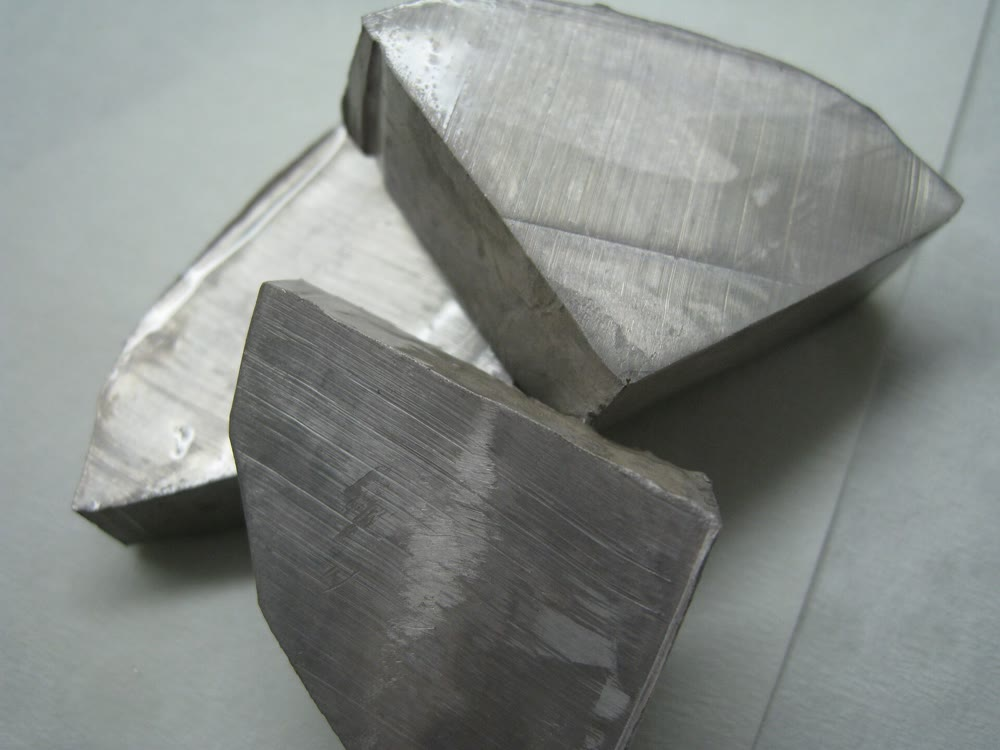
\includegraphics[width=\linewidth,height=4.4cm,keepaspectratio]{images/book1/sodium.jpg}

{\small Le sodium, un \omterm{def:g10:electron-shells:family}{métal alcalin}, coupé au couteau~: mou et argenté
quand il est frais, il se ternit aussitôt à l'\omterm{def:g4:air-a-mixture-of-gases:air}{air}. Photo~: Dnn87,
CC BY-SA 3.0.}
\end{minipage}\hfill
\begin{minipage}[b]{0.48\linewidth}\centering
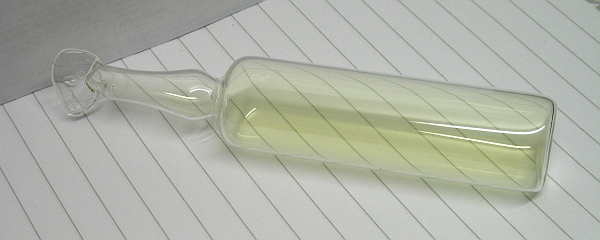
\includegraphics[width=\linewidth,height=4.4cm,keepaspectratio]{images/book1/chlorine-ampoule.jpg}

{\small Le dichlore, un \omterm{def:g10:electron-shells:family}{halogène}~: un gaz jaune-vert, ici scellé dans une
ampoule de verre. Photo~: W.~Oelen, CC BY-SA 3.0.}
\end{minipage}
\end{omfigure}

\begin{inthelab}[Le sodium dans l'eau]
Derrière un écran, l'enseignant laisse tomber un morceau de sodium de la
taille d'un grain de riz dans une grande cuvette d'eau. Il flotte, fond
en une bille brillante et file en tous sens en pétillant, jusqu'à
disparaître~; le gaz dégagé est du dihydrogène, et l'eau restante est
basique.
\end{inthelab}

\begin{safety}{\ghs[0.75cm]{GHS02}\ghs[0.75cm]{GHS05}\quad\ghs[0.75cm]{GHS03}\ghs[0.75cm]{GHS06}}
% ledger: ghs:Na, ghs:Cl2
Le sodium libère du dihydrogène inflammable au contact de l'eau (GHS02)
et provoque de graves brûlures (GHS05). Le dichlore est un gaz comburant
(GHS03), toxique par inhalation (GHS06), également irritant et très
toxique pour les organismes aquatiques. Seul l'enseignant manipule l'un
et l'autre.
\end{safety}

\section{Ions stables et règle des gaz nobles}

\begin{definition}[Règles du duet et de l'octet]\label{def:g10:electron-shells:octet}
Les \omterm{def:g10:electron-shells:family}{gaz nobles}, dont la \omterm{def:g10:electron-shells:configuration}{couche} externe est complète, ne réagissent
presque pas~: leur configuration est particulièrement stable. Quand les
\omterm{def:g7:atoms-and-molecules:atom}{atomes} des premiers éléments forment des \omterm{def:g9:ions:ion}{ions}, ils gagnent ou perdent
des \omterm{def:g9:inside-the-atom:nucleus}{électrons} de façon à acquérir la configuration du \omterm{def:g10:electron-shells:family}{gaz noble} le plus
proche~: deux \omterm{def:g9:inside-the-atom:nucleus}{électrons} dans la \omterm{def:g10:electron-shells:configuration}{couche} 1, comme l'hélium, pour les
\omterm{def:g7:atoms-and-molecules:atom}{atomes} les plus légers --- c'est la \emph{règle du duet}\index{regle du duet@règle du duet} ---,
et huit \omterm{def:g9:inside-the-atom:nucleus}{électrons} sur la \omterm{def:g10:electron-shells:configuration}{couche} externe, comme le néon ou l'argon, pour
les autres --- c'est la \emph{règle de l'octet}\index{regle de l'octet@règle de l'octet}.
\end{definition}

\begin{example}[Les ions prévus par la règle]\label{ex:g10:electron-shells:ions}
Le sodium, $2.8.1$, perd son unique \omterm{def:g10:electron-shells:valence}{électron de valence}~: \ce{Na+},
$2.8$, comme le néon. Le magnésium, $2.8.2$, en perd deux~:
\ce{Mg^{2+}}. L'aluminium, $2.8.3$, en perd trois~: \ce{Al^{3+}}. Le
chlore, $2.8.7$, en gagne un~: \ce{Cl-}, $2.8.8$, comme l'argon.
L'oxygène, $2.6$, en gagne deux~: \ce{O^{2-}}. Le soufre, $2.8.6$~:
\ce{S^{2-}}. Le lithium, $2.1$, en perd un et garde $2$, comme
l'hélium~: \ce{Li+}.
\end{example}

\begin{omfigure}
\begin{tikzpicture}[font=\small]
  \foreach \x/\nm/\cfg/\col in {0/{Na}/{$1\mathrm{s}^2\,2\mathrm{s}^2\,2\mathrm{p}^6\,3\mathrm{s}^1$}/omDef,
      5.8/{\ce{Na+}}/{$1\mathrm{s}^2\,2\mathrm{s}^2\,2\mathrm{p}^6$}/omProp,
      11.0/{Ne}/{$1\mathrm{s}^2\,2\mathrm{s}^2\,2\mathrm{p}^6$}/gray} {
    \node[draw=\col, fill=\col!6, rounded corners=2pt, align=center, text width=3.4cm]
      at (\x,0) {\textbf{\nm}\\ \cfg};
  }
  \draw[->, thick, omProp] (2.0,0) -- (3.8,0) node[midway, above, font=\footnotesize] {perd 1 \ce{e-}};
  \node at (8.4,0) {$=$};
  \node[font=\footnotesize, align=center] at (8.4,-0.75) {même\\ configuration};
\end{tikzpicture}

{\small L'\omterm{def:g9:ions:ion}{ion} sodium a la configuration du néon, le \omterm{def:g10:electron-shells:family}{gaz noble} le plus
proche.}
\end{omfigure}

\begin{remark}[Les limites de la règle]\label{rem:g10:electron-shells:limits}
La règle fonctionne bien pour les vingt premiers éléments et leurs \omterm{def:g9:ions:ion}{ions}
simples. Beaucoup d'éléments, comme le fer (\ce{Fe^{2+}} et
\ce{Fe^{3+}}), ne la suivent pas~; les raisons, et une meilleure
description des \omterm{def:g9:inside-the-atom:nucleus}{électrons}, sont données dans le volume de première
année d'université.
\end{remark}

\section{Exercices}

\begin{exercise}[$\star$]\label{exo:g10:electron-shells:1}
Écrire les \omterm{def:g10:electron-shells:configuration}{configurations électroniques} du carbone ($Z = 6$), de l'azote
($Z = 7$) et du magnésium ($Z = 12$).
\end{exercise}

\begin{exercise}[$\star$]\label{exo:g10:electron-shells:2}
Combien d'\omterm{def:g10:electron-shells:valence}{électrons de valence} le carbone, l'azote et le magnésium
possèdent-ils~?
\end{exercise}

\begin{exercise}[$\star$]\label{exo:g10:electron-shells:3}
Dans quelle \omterm{def:g9:periodic-table-first-look:period}{période} et dans quel groupe se trouve l'élément de
configuration
$1\mathrm{s}^2\,2\mathrm{s}^2\,2\mathrm{p}^6\,3\mathrm{s}^2\,3\mathrm{p}^3$~?
\end{exercise}

\begin{exercise}[$\star$]\label{exo:g10:electron-shells:4}
Nommer les trois familles de ce chapitre et donner deux éléments de
chacune.
\end{exercise}

\begin{exercise}[$\star$]\label{exo:g10:electron-shells:5}
Énoncer la \omterm{def:g10:electron-shells:octet}{règle de l'octet}.
\end{exercise}

\begin{exercise}[$\star\star$]\label{exo:g10:electron-shells:6}
À l'aide de la règle des \omterm{def:g10:electron-shells:family}{gaz nobles}, donner l'\omterm{def:g9:ions:ion}{ion} formé par le potassium
($Z = 19$) et par le fluor ($Z = 9$), avec leurs configurations.
\end{exercise}

\begin{exercise}[$\star\star$]\label{exo:g10:electron-shells:7}
Un élément a 2 \omterm{def:g9:inside-the-atom:nucleus}{électrons} dans sa troisième \omterm{def:g10:electron-shells:configuration}{couche}, qui est sa \omterm{def:g10:electron-shells:configuration}{couche}
externe. Donner sa configuration, son \omterm{def:g9:inside-the-atom:atomic-number}{numéro atomique} et son nom.
\end{exercise}

\begin{exercise}[$\star\star$]\label{exo:g10:electron-shells:8}
À l'aide des \omterm{def:g9:ions:ion}{ions} stables, écrire la formule du \omterm{def:g9:ions:ionic-compound}{composé ionique} formé par
le magnésium et le chlore, puis par l'aluminium et l'oxygène.
\end{exercise}

\begin{exercise}[$\star\star$]\label{exo:g10:electron-shells:9}
Observer le tableau des vingt premiers éléments. Quels éléments ont le
même nombre d'\omterm{def:g10:electron-shells:valence}{électrons de valence} que l'oxygène~?
\end{exercise}

\begin{exercise}[$\star\star$]\label{exo:g10:electron-shells:10}
Expliquer pourquoi le néon, contrairement au sodium et au chlore, ne
forme pas d'\omterm{def:g9:ions:ion}{ions} au cours des \omterm{def:g7:chemical-reactions:reaction}{réactions chimiques}.
\end{exercise}

\begin{exercise}[$\star\star$]\label{exo:g10:electron-shells:11}
L'\omterm{def:g9:ions:ion}{ion} \ce{X^{2+}} a la configuration de l'argon. Identifier $X$.
\end{exercise}

\begin{exercise}[$\star\star\star$]\label{exo:g10:electron-shells:12}
L'hélium a 2 \omterm{def:g10:electron-shells:valence}{électrons de valence}, mais il est placé dans le \omterm{def:g9:periodic-table-first-look:period}{groupe} 18,
et non dans le \omterm{def:g9:periodic-table-first-look:period}{groupe} 2. Expliquer à l'aide de sa configuration.
\end{exercise}

\begin{exercise}[$\star\star\star$]\label{exo:g10:electron-shells:13}
Le potassium réagit avec l'eau encore plus violemment que le sodium. À
l'aide de la distance entre l'\omterm{def:g10:electron-shells:valence}{électron de valence} et le \omterm{def:g9:inside-the-atom:nucleus}{noyau}, proposer
une explication.
\end{exercise}

\begin{exercise}[$\star\star\star$]\label{exo:g10:electron-shells:14}
Donner les configurations de \ce{S^{2-}}, \ce{Cl-}, \ce{K+} et
\ce{Ca^{2+}}. Qu'ont-elles en commun~?
\end{exercise}

\begin{exercise}[$\star\star\star$]\label{exo:g10:electron-shells:15}
Un élément de la \omterm{def:g9:periodic-table-first-look:period}{période} 3 forme l'\omterm{def:g9:ions:ion}{ion} \ce{Y^{3-}}. Déterminer son
groupe, sa configuration et son nom.
\end{exercise}

\section{Problème~: rubis, saphir et corindon}

\begin{problem}[{Problème du week-end --- les électrons derrière une pierre
précieuse~: de deux configurations au nombre d'électrons déplacés dans un
gramme}]
\label{pb:g10:electron-shells:1}
Les rubis et les saphirs sont des formes gemmes du corindon, un \omterm{def:g9:ions:ionic-compound}{composé
ionique} d'aluminium et d'oxygène~; une trace d'autres métaux leur donne
leurs couleurs. Le corindon est assez dur pour rayer presque tout, et le
corindon en poudre sert à polir les lentilles. On prendra pour masse
d'un \omterm{def:g9:inside-the-atom:proton}{nucléon} \qty{1.67e-27}{kg}~; l'aluminium~27 compte 27 \omterm{def:g9:inside-the-atom:proton}{nucléons},
l'oxygène~16 en compte 16.

\medskip
\noindent\textbf{Partie I --- Les \omterm{def:g7:atoms-and-molecules:atom}{atomes}.}
\begin{enumerate}
  \item Donner les nombres de \omterm{def:g9:inside-the-atom:proton}{protons} et d'\omterm{def:g9:inside-the-atom:nucleus}{électrons} d'un \omterm{def:g7:atoms-and-molecules:atom}{atome}
        d'aluminium ($Z = 13$) et d'un \omterm{def:g7:atoms-and-molecules:atom}{atome} d'oxygène ($Z = 8$).
  \item Écrire leurs \omterm{def:g10:electron-shells:configuration}{configurations électroniques}.
  \item Combien d'\omterm{def:g10:electron-shells:valence}{électrons de valence} chacun possède-t-il~? Dans quelle
        \omterm{def:g9:periodic-table-first-look:period}{période} et dans quel groupe se trouve chacun~?
  \item L'aluminium est-il un \omterm{def:g9:periodic-table-first-look:metal}{métal} ou un \omterm{def:g9:periodic-table-first-look:metal}{non-métal}~? Et l'oxygène~?
\end{enumerate}

\medskip
\noindent\textbf{Partie II --- Les \omterm{def:g9:ions:ion}{ions}.}
\begin{enumerate}[resume]
  \item À l'aide de la \omterm{def:g10:electron-shells:octet}{règle de l'octet}, déterminer l'\omterm{def:g9:ions:ion}{ion} que forme
        l'aluminium. Écrire sa configuration.
  \item Quel \omterm{def:g9:ions:ion}{ion} l'oxygène forme-t-il~? Écrire sa configuration.
  \item Quel \omterm{def:g10:electron-shells:family}{gaz noble} a la même configuration que ces deux \omterm{def:g9:ions:ion}{ions}~?
  \item Combien d'\omterm{def:g9:inside-the-atom:nucleus}{électrons} un \omterm{def:g7:atoms-and-molecules:atom}{atome} d'aluminium perd-il, et combien un
        \omterm{def:g7:atoms-and-molecules:atom}{atome} d'oxygène en gagne-t-il~?
\end{enumerate}

\medskip
\noindent\textbf{Partie III --- La formule.}
\begin{enumerate}[resume]
  \item Trouver la formule du corindon, le composé neutre formé par ces
        \omterm{def:g9:ions:ion}{ions}.
  \item Dans une unité de formule, combien d'\omterm{def:g9:inside-the-atom:nucleus}{électrons} sont perdus par les
        \omterm{def:g7:atoms-and-molecules:atom}{atomes} d'aluminium~? Gagnés par les \omterm{def:g7:atoms-and-molecules:atom}{atomes} d'oxygène~?
  \item Pourquoi ces deux nombres doivent-ils être égaux~?
  \item Un rubis contient une trace d'\omterm{def:g9:ions:ion}{ions} chrome \ce{Cr^{3+}} à la place
        de certains \omterm{def:g9:ions:ion}{ions} \ce{Al^{3+}}. Pourquoi un \omterm{def:g9:ions:ion}{ion} \ce{Cr^{3+}}
        peut-il prendre la place d'un \omterm{def:g9:ions:ion}{ion} \ce{Al^{3+}} sans perturber
        les charges~?
\end{enumerate}

\medskip
\noindent\textbf{Partie IV --- Un gramme de corindon.}
\begin{enumerate}[resume]
  \item Combien de \omterm{def:g9:inside-the-atom:proton}{nucléons} y a-t-il dans une unité de formule de
        corindon~?
  \item Calculer la masse d'une unité de formule (\omterm{def:g9:inside-the-atom:nucleus}{électrons} négligés).
  \item Combien d'unités de formule y a-t-il dans \qty{1}{g} de
        corindon~?
  \item Combien d'\omterm{def:g9:ions:ion}{ions} \ce{Al^{3+}} et d'\omterm{def:g9:ions:ion}{ions} \ce{O^{2-}} cela
        représente-t-il~?
  \item Pourquoi peut-on négliger les \omterm{def:g9:inside-the-atom:nucleus}{électrons} à la question 14~?
  \item Combien d'\omterm{def:g9:inside-the-atom:nucleus}{électrons} ont été transférés de l'aluminium à
        l'oxygène pour former \qty{1}{g} de corindon~?
\end{enumerate}
\end{problem}
